\chapter*{Appendix A} 
\addcontentsline{toc}{chapter}{Appendix A}
\markboth{Appendix A}{Appendix A}
\label{app:AppendixA}

A more accurate description of the resonance profile for a two-dimensional notch-type resonator is provided in the literature \cite{Gao2008}, where the transmitted signal is modeled as a complex function of frequency. 
The complete expression for the complex transmission coefficient is given by

\begin{equation}
S_{21}(f) = ae^{i\alpha}e^{-2\pi i f \tau}\left[ 1 - \frac{(Q_l/|Q_c|)e^{i\phi}}{1 + 2iQ_l(f/f_r -1)} \right].
\end{equation}

This formulation provides a deeper insight into both the environmental and resonator-specific contributions to the observed response. 
The prefactor accounts for the attenuation and gain in the measurement chain through the amplitude $a$, introduces a global phase shift $\alpha$, and models the effect of finite cable length via a frequency-dependent delay term characterized by the parameter $\tau$. 
These components collectively represent systematic effects that shape the baseline response of the system.

The second part of the expression captures the physical behavior of the resonator itself. 
It includes the loaded quality factor $Q_l$, which reflects the total energy loss in the system, and the coupling quality factor $Q_c$, which quantifies the interaction between the resonator and the transmission line. 
The resonance frequency $f_r$ marks the center of the frequency response, while the phase offset $\phi$ accounts for impedance mismatches and Fano-type interferences caused by reflections within the setup.
This model exploits all the information encoded in both the magnitude and phase of the complex transmission signal, allowing for a more comprehensive characterization. 

\paragraph{}
However, directly fitting the complete model involves a nonlinear optimization over seven parameters, which is inherently sensitive to initial conditions and often non-robust. 
To improve the stability and reliability of the fitting process, the problem is decomposed and approached in stages, each targeting a subset of parameters.

First, the cable delay is estimated by fitting a linear function to the phase response across frequency. 
The delay introduces a phase tilt proportional to the frequency, and its removal reveals the underlying circular shape of the resonance response in the complex plane. 
Once the delay is corrected, a geometric circle fit is performed on the data.

Then the phase angle $\theta$ is fit according to the following expression:
\begin{equation}
    \theta(f) = \theta_0 - 2\pi \tau (f - f_r) + 2 \arctan \left[ 2 Q_l \left( 1 - \frac{f}{f_r} \right) \right],
\end{equation}
where an additional linear term accounts for any residual cable delay not captured in the initial correction. 
This protocol is implemented in \Qibocal and available by selecting the \tt{s21} fitting routine for the resonator spectroscopy, an example of the expected output obtained from running such experiment is shown in Figure \ref{fig:res_s21}.

\begin{figure}[ht!]
    \centering
    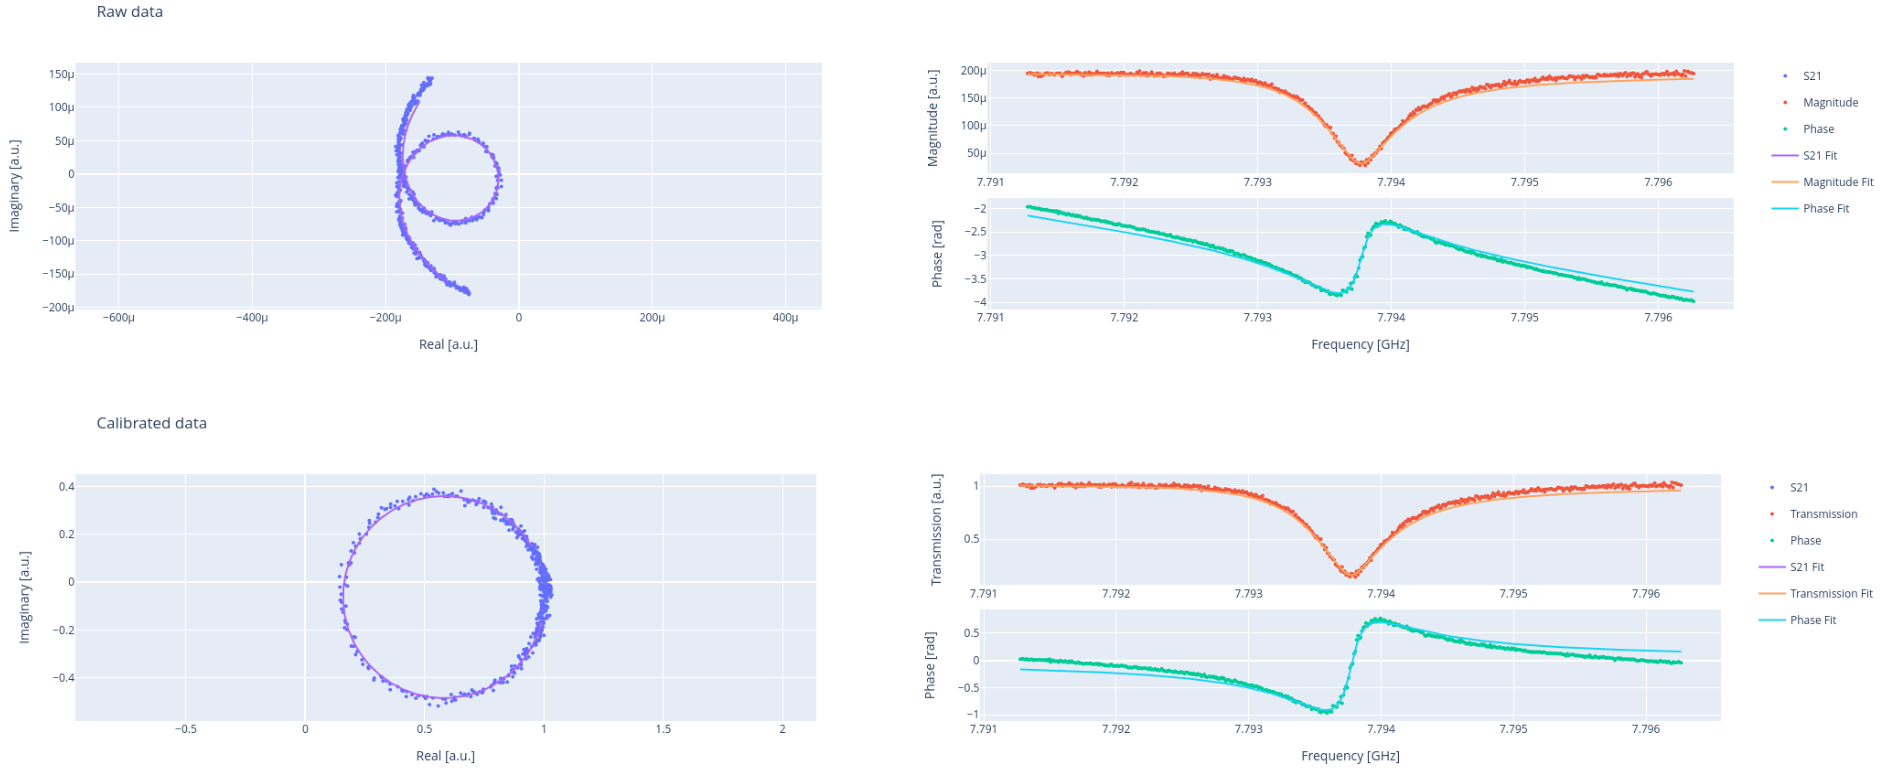
\includegraphics[width=\textwidth]{figures/png/s21.png}
    \caption{Output of resonator spectroscopy performed with \tt{s21} fit function.}
    \label{fig:res_s21}
\end{figure}

\chapter*{Appendix B}
\addcontentsline{toc}{chapter}{Appendix B}
\markboth{Appendix B}{Appendix B}
\label{app:AppendixB}

In general, it is possible to show that for different forms of the detuning flux 
\begin{equation}\label{eq:det_flux}
    \Delta f(\Phi) = a\Phi^k
\end{equation}
where $k \in \mathbb{Z}^+$, the relative phase $\varphi_{\tau}$ can be calculated as follows:
\begin{align}
    \varphi_\tau &= 2\pi a \int_{0}^{\infty} \left[ \int_{0}^{\infty} h(t - t') dt' - \int_{0}^{\infty} h(t - \tau - t') dt' \right]^k dt \\
    &= 2\pi a \int_{0}^{\tau} \left[ \int_{0}^{t} h(t - t') dt' \right]^k dt + 2\pi a \int_{\tau}^{\infty} \left[ \int_{0}^{\tau} h(t - t') dt' \right]^k dt,
\end{align}

From the calculations showed in \ref{eq:phi} we know that the relative phase $\varphi_\tau$ for a general form of the detuning flux \ref{eq:det_flux}, with $T_{\text{sep}} = \infty$ is
\begin{equation}\label{eq:phi_here}
    \varphi_{\tau} = 2\pi \int_{0}^{+\infty} a \left[ \left( s(t) - s(t - \tau) \right) \right]^k dt = 2\pi a \int_{0}^{+\infty} \left[ \left( s(t) - s(t - \tau) \right) \right]^k dt
\end{equation}

As hypothesis we know that voltage-to-flux step response of the control line is 
\begin{equation}\label{eq:voltage_to_flux}
    s(t) = \left(1 - e^{-t/\tau} \right) \cdot u(t),
\end{equation} where $u(t)$ is the step function, and that the impulse response is 
\begin{equation}\label{eq:h_def}
    h(t) = \frac{\text{d}s}{\text{d}t}
\end{equation}


If we substitute the expression of $s(t)$ given in \ref{eq:voltage_to_flux} in equation \ref{eq:phi_here} we obtain
\begin{equation}\label{eq:first_step_dem}
    \varphi_{\tau} = 2\pi a \int_{0}^{+\infty} \left[ \int_{0}^{+\infty} h(t - t') dt' - \int_{0}^{+\infty} h(t - \tau - t') dt' \right]^k dt.
\end{equation}

To do we have to show that \begin{enumerate}
    \item \begin{equation}\label{eq:first_dem}
        s(t) = \int_0^{+\infty} h(t-t')dt'
    \end{equation}
    \item \begin{equation}\label{eq:sec_dem}
        s(t-\tau) = \int_{0}^{+\infty} h(t-\tau-t')dt'
    \end{equation}
\end{enumerate}

We start from the demonstration of equation \ref{eq:first_dem}. By definition \ref{eq:h_def} we can write
\begin{equation}\label{eq:first_dem1}
    h(t) = \frac{d}{dt} \left[ \left(1 - e^{-t/\tau} \right) u(t) \right] = \frac{e^{-t/\tau}}{\tau} u(t) + \left(1 - e^{-t/\tau} \right) \delta(t), 
\end{equation}

substituting Eq \ref{eq:first_dem1} in Eq \ref{eq:first_dem} we obtain \begin{equation}
    \int_{0}^{+\infty} h(t - t') dt' = \int_{0}^{+\infty} \frac{e^{-\frac{(t - t')}{\tau}}}{\tau} u(t - t') dt' + \int_{0}^{+\infty} \left(1 - e^{-(t - t')/\tau} \right) \delta(t - t') dt',
\end{equation}
by setting $t'' = t-t'$, $dt''=-dt'$,  we have $t''\rightarrow -\infty$ for $t'\rightarrow +\infty$ and $t''= t$ for $t'= 0$, the integral then becomes
\begin{align}
    \int_{0}^{+\infty} h(t - t') dt' &= \int_{t}^{-\infty} -\frac{e^{-t''/\tau}}{\tau} u(t'') dt'' - \int_{t}^{-\infty} \left(1 - e^{-t''/\tau} \right) \delta(t'') dt'' \\
    &= \int_{-\infty}^{t} \frac{e^{-t''/\tau}}{\tau} u(t'') dt'' + \int_{-\infty}^{t} \left(1 - e^{-t''/\tau} \right) \delta(t'') dt''\\
    &= \int_{0}^{t} \frac{e^{-t''/\tau}}{\tau} u(t'') dt'' + \left(1 - e^{-t''/\tau} \right) \Big|_{t''=0}\\
    &= \left[ -e^{-t''/\tau} u(t'') \right]_{0}^{t} + 0\\
    &= (1 - e^{-t/\tau}) u(t)\\
\end{align}
that concludes the demonstration of Eq \ref{eq:first_dem}.
To demonstrate equation \ref{eq:sec_dem} we starting again by using the definition of $s(t)$ to compute 
\begin{align}
    h(t -t'-\tau) &= \frac{d}{dt} \left[ \left(1 - e^{-(t-t'-\tau)/\tau} \right) u(t-t'-\tau) \right] \\
    &= \frac{e^{-(t-t'-\tau)/\tau}}{\tau} u(t-t'-\tau) + \left(1 - e^{-(t-t'-\tau)/\tau} \right) \delta(t-t'-\tau)\\ \label{eq:sec_dem2}
\end{align}

We can substitute \ref{eq:sec_dem2} in equation \ref{eq:sec_dem} and obtain \begin{equation}
    \int_{0}^{+\infty} h(t - t' - \tau) \, dt' = \int_{0}^{+\infty} \frac{e^{-(t - t' - \tau)/\tau}}{\tau} u(t - t' - \tau) dt' + \int_{0}^{+\infty} \left(1 - e^{-(t - t' - \tau)/\tau} \right) \delta(t - t' - \tau) dt'
\end{equation}
by setting $t'' = t-t'-\tau$, $dt''=-dt'$,  we have $t''\rightarrow -\infty$ for $t'\rightarrow +\infty$ and $t'' = t-\tau$ for $t'= 0$, the integral then becomes
\begin{align}
    \int_{0}^{+\infty} h(t - t'-\tau) dt' &= \int_{-\infty}^{t - \tau} \frac{-e^{-t''/\tau}}{\tau} u(t'') dt'' - \int_{t - \tau}^{\infty} (1 - e^{-t''/\tau}) \delta(t'')\\
    &= \int_{-\infty}^{t - \tau} \frac{e^{-t''/\tau}}{\tau} u(t'') dt'' + \int_{-\infty}^{t - \tau} (1 - e^{-t''/\tau}) \delta(t'')\\
    &= \int_{0}^{t - \tau} \frac{e^{-t''/\tau}}{\tau} u(t'') dt'' + \left(1 - e^{-t''/\tau} \right) \Big|_{t''=0}\\
    &= \left[ - e^{-t''/\tau} u(t'') \right]_{0}^{t - \tau} + 0\\
    &= (1 - e^{-t''/\tau}) u(t'')\\
    &= s(t'') = s(t - t' - \tau)
\end{align}

With this, we demonstrated that 
\begin{equation}
    \varphi_\tau = 2\pi a \int_{0}^{\infty} \left[ \int_{0}^{\infty} h(t - t') \, dt' - \int_{0}^{\infty} h(t - \tau - t') dt' \right]^k dt ,
\end{equation}

We now need to show that 
\begin{align}\label{eq:second_step_dem}
    &2\pi a \int_{0}^{\infty} \left[ \int_{0}^{\infty} h(t - t') dt' - \int_{0}^{\infty} h(t - \tau - t') dt' \right]^k dt\\ 
    &= 2\pi a \int_{0}^{\tau} \left[ \int_{0}^{t} h(t - t') dt' \right]^k dt + 2\pi a \int_{\tau}^{\infty} \left[ \int_{0}^{\tau} h(t - t') \, dt' \right]^k dt.
\end{align}
%
As first step we can try to rewrite the left-hand-side (LHS) in a different way:
\begin{align}
    & 2\pi a \int_{0}^{\infty} \left[ \int_{0}^{\infty} h(t - t') dt' - \int_{0}^{\infty} h(t - \tau - t') dt' \right]^k dt\\ \label{eq:last1}
    &= 2\pi a \int_{0}^{\infty} \left[s(t) -s(t-\tau)\right]^k dt\\ \label{eq:last2}
    &= 2\pi\alpha \int_0^{+\infty} \left[\left(1 - e^{-t/\tau}\right) u(t) - \left(1 - e^{-(t - \tau)/\tau}\right) u(t - \tau)\right]^k dt\\ \label{eq:last3}
    &= 2\pi\alpha \int_0^{\tau} \left[ \left(1 - e^{-t/\tau}\right)u(t)\right]^k dt + 2\pi\alpha \int_{\tau}^{+\infty} \left[ \left(1 - e^{-t/\tau}\right)u(t) - \left(1 - e^{-(t - \tau)/\tau}\right)u(t-\tau) \right]^k dt\\ \label{eq:last4}
    &=  2\pi\alpha \int_0^{\tau} \left[\int_{0}^{\infty} h(t - t') dt' \right]^k dt + 2\pi\alpha \int_{\tau}^{+\infty} \left[ s(t) - s(t-\tau) \right]^k dt\\ \label{eq:last_step}
\end{align}
%
In the first step, to get equation \ref{eq:last2} I simply used the equations \ref{eq:first_dem} and \ref{eq:sec_dem} that were demonstarted before, then by substituting the definition of $s(t)$ we obtain Eq \ref{eq:last3}.
It is possible to separate the integral in equation \ref{eq:last3} by using the definition of $u(t)$ which is null for $t\tau$ and of $u(t-\tau)$ which is null also for $0<t<\tau$, doing this we obtain Eq, \ref{eq:last4}
By substituting back \ref{eq:first_dem} in the first term of equation \ref{eq:last4} we obtain the first term of equation \ref{eq:second_step_dem} which we want to demonstrate, in the second term of the sum instead, we can substitute back the definition of $s(t)$.

At this point we only have to show that for $t>\tau$, which is the interval we are considering in the second term, 
\begin{equation}
    2\pi\alpha \int_{\tau}^{+\infty} \left[ s(t) - s(t-\tau) \right]^k dt = 2\pi a \int_{\tau}^{\infty} \left[ \int_{0}^{\tau} h(t - t') dt' \right]^k dt.
\end{equation}
%
To do this we can first evaluate $s(t)-s(t-\tau)$ in the interval $t>\tau$ so that $u(t)=u(t-\tau)=1$, we have
\begin{equation}\label{eq:final}
    s(t) - s(t-\tau) = 1- e^{-\frac{t}{\tau}} - 1 + e^{-\frac{(t-\tau)}{\tau}} = e^{-\frac{t}{\tau}} \left(e^{\frac{\tau}{\tau}}-1\right) = (e-1)e^{-\frac{t}{\tau}}
\end{equation}
%
If we then compute $\int_{0}^{\tau} h(t - t')dt'$ we obtain
\begin{align}
    \int_{0}^{\tau} h(t-t')dt' &= \int_{0}^{\tau} \left[ \frac{e^{-\frac{(t-t')}{\tau}}}{\tau} u(t-t') - \left(1-e^{-\frac{t-t'}{\tau}}\right)\delta(t-t') \right] dt'\\
    &= \int_{0}^{\tau} \frac{e^{-\frac{(t-t')}{\tau}}}{\tau} u(t-t')dt' \\
    &= \int_{0}^{\tau} \frac{e^{-\frac{(t-t')}{\tau}}}{\tau} dt'\\
    &= \int_{0}^{\tau} \frac{e^{-\frac{t}{\tau}}e^{\frac{t'}{\tau}}}{\tau} = e^{-\frac{t}{\tau}}e^{\frac{t'}{\tau}}\Big|_{0}^{\tau} = e^{\frac{-t}{tau}}(e-1)
\end{align}
which is equal to \ref{eq:final} and then concludes the demonstration.

\chapter*{Appendix C}
\addcontentsline{toc}{chapter}{Appendix C}
\markboth{Appendix C}{Appendix C}
\label{app:AppendixC}

In this appendix are reported the plots of all the Randomized Benchmarking evaluations that have been performed during the optimization using different optimization methods.
\begin{figure}[h!]
    \centering
    \begin{subfigure}[t]{0.45\textwidth}
        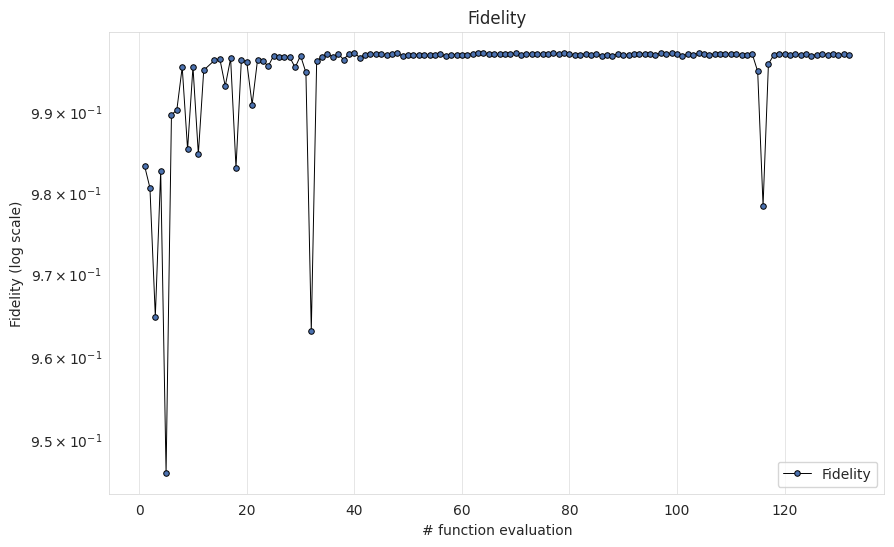
\includegraphics[width=\textwidth]{figures/png/RB_optimization/NM/post_ft_true/NM_complete.png}
        \caption{Plot of the avarge Clifford gate fidielity as a function of the function evauluations. First optimization attempt with Nelder-Mead algorithm.}
        \label{NM_true_fig:complete}
    \end{subfigure}
    \hfill
    \begin{subfigure}[t]{0.45\textwidth}
        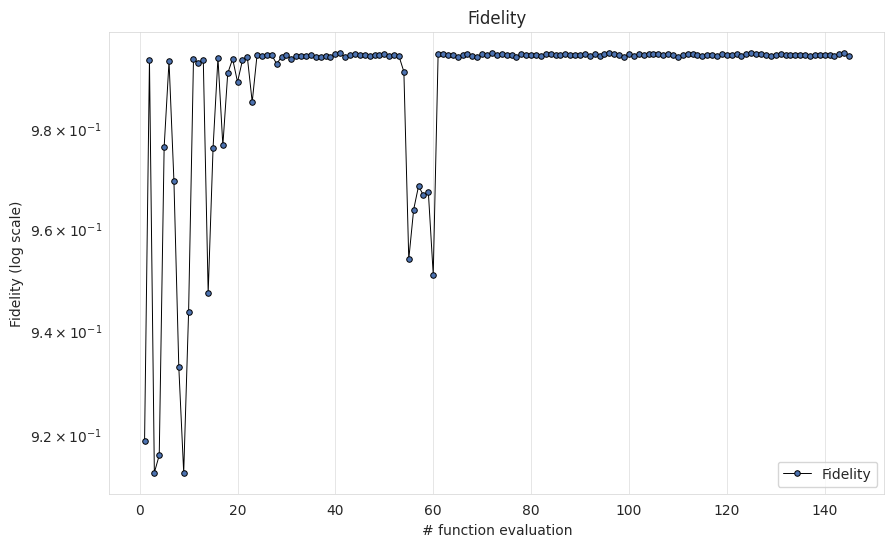
\includegraphics[width=\textwidth]{figures/png/RB_optimization/NM/InitialSymplex/20241110_211211/complete.png}
        \caption{Plot of the avarge Clifford gate fidielity as a function of the function evauluations.\\
                Optimization method: Nelder-Mead algorithm with initial symplex - \tt{init\_symp\_1}.}
        \label{NM_true_fig:}
    \end{subfigure}

    \vspace{0.5cm}

    \begin{subfigure}[t]{0.45\textwidth}
        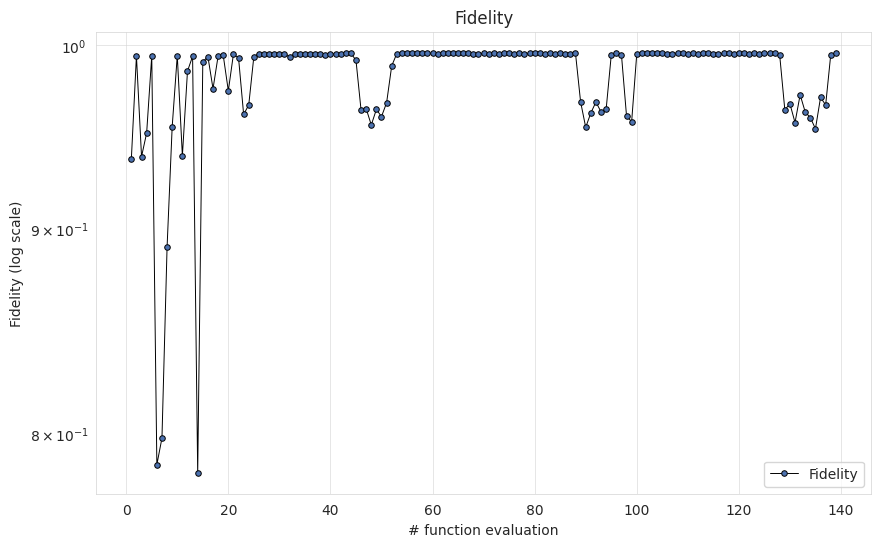
\includegraphics[width=\textwidth]{figures/png/RB_optimization/NM/InitialSymplex/20241113_181711/complete.png }
        \caption{Plot of the avarge Clifford gate fidielity as a function of the function evauluations.\\
                Optimization method: Nelder-Mead algorithm with initial symplex - \tt{init\_symp\_2}.}
        \label{NM_true_fig:}
    \end{subfigure}
    \hfill
    \begin{subfigure}[t]{0.45\textwidth}
        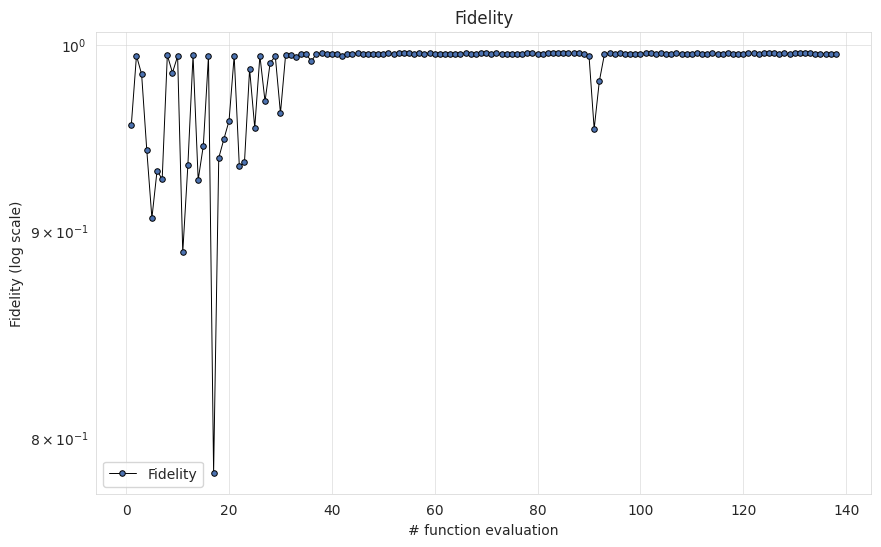
\includegraphics[width=\textwidth]{figures/png/RB_optimization/NM/InitialSymplex/20241113_200745/complete.png}
        \caption{Plot of the avarge Clifford gate fidielity as a function of the function evauluations.\\
                Optimization method: Nelder-Mead algorithm with initial symplex - \tt{init\_symp\_3}.}
        \label{NM_true_fig:}
    \end{subfigure}

    \caption{Plots of the fidelity and optimization parameters as a function of the number of optimization step.}
    \label{fig:complete}
\end{figure}

\chapter*{Appendix D}
\addcontentsline{toc}{chapter}{Appendix D}
\markboth{Appendix D}{Appendix D}
\label{app:AppendixD}

In quantum computing, measurements are restricted to the computational basis, corresponding to projective measurements along the $z$-axis of the Bloch sphere. 
As a result, direct access is limited to determining the probability of a qubit being in the $\ket{0}$ or $\ket{1}$ state.
To extract information about other components of the qubit state, such as its projections along the $x-$ or $y-$ axes, indirect measurement techniques are required. 
These involve applying single-qubit rotations that map the desired observable onto the $z-$axis before the readout.
For example, in the cryoscope experiment we need to measure $\langle X \rangle$ and $\langle Y \rangle$ in order to then access the relative phase information.
 
\paragraph{$\langle X \rangle$ measurement}
To measure $\langle X \rangle$, we begin by applying a $\frac{\pi}{2}$ rotation around the $y$-axis, which transforms the ground state $\ket{0}$ into the superposition state $\ket{0}$ a $\frac{(\ket{0} + \ket{1})}{\sqrt{2}}$.
Next, a flux pulse of duration $\tau$ is applied, introducing a phase $\varphi_\tau$ between the computational basis states. After this evolution, the qubit state become $\ket{\psi}=\frac{\ket{0} + e^{i\varphi_\tau} \ket{1}}{\sqrt{2}}$.

The expectation value of the Pauli $X$ operator in this state is:
\begin{align}
    \langle X \rangle &= \left( \frac{\bra{0} + e^{- i\varphi_\tau} \bra{1}}{\sqrt{2}} \right) \hat{\sigma}_x \left( \frac{\ket{0} + e^{ i \varphi_\tau} \ket{1}}{\sqrt{2}} \right)\\
    &= \left( \frac{\bra{0} + e^{- i \varphi_\tau} \bra{1}}{\sqrt{2}} \right)\left( \frac{\ket{1} + e^{ i \varphi_\tau} \ket{0}}{\sqrt{2}} \right)\\
    &= \frac{e^{ i \varphi_\tau} + e^{- i\varphi_\tau}}{2} = \cos{(\varphi_\tau)}.
\end{align}

Since the measurement can only be performed along the $z$-axis, we apply a rotation $R_Y(\frac{\pi}{2})$ to map the $x$-axis component onto the $z$-axis. The operator for this rotation is
\begin{align}\label{eq:RY90}
    R_Y(\frac{\pi}{2}) &= \exp{\left( -i\frac{\pi}{4}\hat{\sigma}_y\right)}\\
    &= \cos{\left(\frac{\pi}{4}\right)}\id - i\sin{\left(\frac{\pi}{4}\right)}\hat{\sigma}_y\\
    &= \frac{\sqrt{2}}{2}(\id -i\hat{\sigma}_y) = \begin{pmatrix}
        1 & -1 \\
        1 & 1
        \end{pmatrix}.
\end{align}

Applying this rotation to the state $\ket{\psi}$ gives:
\begin{equation}
    \ket{\psi'} = R_Y\left(\frac{\pi}{2}\right) \ket{\psi} = \frac{1}{\sqrt{2}} 
\begin{pmatrix}
1 & -1 \\
1 & 1
\end{pmatrix}
\frac{1}{\sqrt{2}} 
\begin{pmatrix}
1 \\
e^{i\varphi_\tau}
\end{pmatrix}
= \frac{1}{2}
\begin{pmatrix}
1 - e^{i\varphi_\tau} \\
1 + e^{i\varphi_\tau}
\end{pmatrix}
\end{equation}

We now measure the probability $p_1$ of finding the qubit in state $\ket{1}$:
\begin{align}\label{eq:P1X}
    p_1 &= |\braket{\psi'|1}|^2 = \left| \frac{1}{2} \left( (1 - e^{i\varphi_\tau})\bra{0} + (1 + e^{i\varphi_\tau})\bra{1} \right) \ket{1} \right|^2 = \left| \frac{1 + e^{i\varphi_\tau}}{2} \right|^2\\
        &= \frac{1}{4} (1+e^{-i\varphi_\tau})(1+e^{+i\varphi_\tau}) = \frac{1}{4}(1 + e^{+i\varphi_\tau} + e^{-i\varphi_\tau} +1)\\ 
        &=\frac{(2+ 2\cos{\varphi_\tau})}{4} = \frac{1 + \cos{\varphi_\tau}}{2}.
\end{align}

Thus, the expectation value $\langle X \rangle$ is recovered via $\langle X \rangle = 2\cdot p_1 - 1$.

\paragraph{$\langle Y \rangle$ measurement}
To measure $\langle Y \rangle$, the same initial sequence is applied: a $\frac{\pi}{2}$ rotation around the $y$-axis followed by a flux pulse of duration $\tau$, leading to the state: $\ket{\psi}=\frac{\ket{0} + e^{i\varphi_\tau} \ket{1}}{\sqrt{2}}$.

The expectation value of the Pauli $Y$ operator is given by:
\begin{align}
    \langle Y \rangle &= \left( \frac{\bra{0} + e^{- i\varphi_\tau} \bra{1}}{\sqrt{2}} \right) \hat{\sigma}_y \left( \frac{\ket{0} + e^{ i \varphi_\tau} \ket{1}}{\sqrt{2}} \right)\\
    &= \left( \frac{\bra{0} + e^{- i \varphi_\tau} \bra{1}}{\sqrt{2}} \right) \left( \frac{\ket{1} + e^{ i \varphi_\tau} \ket{0}}{\sqrt{2}} \right)\\
    &= \frac{e^{ i \varphi_\tau} - e^{- i\varphi_\tau}}{2} = \sin{(\varphi_\tau)}
\end{align}

To access this observable through a $z$-axis measurement, we apply a rotation $R_X(\frac{\pi}{2})$:
\begin{align}\label{eq:RX90}
    R_X(\frac{\pi}{2}) &= \exp{\left( -i\frac{\pi}{4}\hat{\sigma}_x\right)}\\
    &= \cos{\left(\frac{\pi}{4}\right)}\id - i\sin{\left(\frac{\pi}{4}\right)}\hat{\sigma}_x\\
    &= \frac{\sqrt{2}}{2}(\id -i\hat{\sigma}_x) = \begin{pmatrix}
        1 & -i \\
        -i & 1
        \end{pmatrix}.
\end{align}

The probability of measuring $\ket{1}$ is:
\begin{equation}
    \ket{\psi'} = R_X\left(\frac{\pi}{2}\right) \ket{\psi} = \frac{1}{\sqrt{2}} 
\begin{pmatrix}
1 & -i \\
-i & 1
\end{pmatrix}
\frac{1}{\sqrt{2}} 
\begin{pmatrix}
1\\
e^{i\varphi_\tau}
\end{pmatrix}
= \frac{1}{2}
\begin{pmatrix}
1 - ie^{i\varphi_\tau} \\
-i + e^{i\varphi_\tau}
\end{pmatrix}
\end{equation}

The probability of measuring $\ket{1}$ is:
\begin{align}\label{eq:P1Y}
    p_1 &= |\braket{1 | \psi'}|^2 = \left| \frac{1}{2} \bra{1} \left( (1 - ie^{i\varphi_\tau})\ket{0} + (-i + e^{i\varphi_\tau})\ket{1} \right) \right|^2 = \left| \frac{-i + e^{i\varphi_\tau}}{2} \right|^2\\
        &= \frac{1}{4} (i+e^{-i\varphi_\tau})(-i+e^{+i\varphi_\tau}) = \frac{1}{4}(1 + -ie^{-i\varphi_\tau} + e^{+i\varphi_\tau} +1)\\ 
        &=\frac{(2- 2\sin{\varphi_\tau})}{4} = \frac{1 -\sin{\varphi_\tau}}{2}.
\end{align}

Therefore, the expectation value $\langle Y \rangle$ can be expressed as $\langle Y \rangle =- 2\cdot p_1 + 1$.


\begin{comment}
Possibili esensioni dell'appendice in ordine di priorità:
* spiegare com'è Qibo
* spiegare come ho gestito il passaggio a ruff
\end{comment}

\chapter*{Appendix E}
\addcontentsline{toc}{chapter}{Appendix E}
\markboth{Appendix E}{Appendix E}
\label{app:AppendixE}

Before running the cryoscope experiment, it is necessary to first execute the \texttt{flux\_amplitude\_frequency} routine. 
The purpose of this routine is to determine the coefficients of the quadratic relationship between the detuning experienced by the qubit and the amplitude of the applied magnetic flux pulse. 
According to equation, \ref{eq:freqdepndenceonflux} This relationship is assumed to take the form:
\begin{equation}
f = c_1 A^2 + c_2 A + c_3,
\label{eq:freqdepndenceonflux}
\end{equation}
where $f$ is the detuning and $A$ is the flux amplitude. 
Knowledge of this relation is essential for later reconstructing the time-dependent flux from the detuning profile extracted in the cryoscope measurement.

The pulse sequence used in this calibration is identical to that of the cryoscope experiment, and measurements are again performed in both the $\langle X(t) \rangle$ and $\langle Y(t) \rangle$ bases. 

However, in this case, the duration of the flux pulse is fixed and specified by the user via the \tt{duration} parameter, while the amplitude of the pulse is swept over a user-defined range. 
This range is set through the \tt{amplitude\_min}, \tt{amplitude\_max}, and \tt{amplitude\_step} parameters defined in the experiment's runcard configuration.

The postprocessing follows a procedure similar to that used for cryoscope data. 
First, the raw measurement probabilities are converted to expectation values by inverting the relations:
\begin{align}
\langle X(t) \rangle &= 2p^X_1(t) - 1, \\
\langle Y(t) \rangle &= 1 - 2p^Y_1(t),
\end{align}
where $p^X_1(t)$ and $p^Y_1(t)$ are the measured probabilities of finding the qubit in the excited state $\ket{1}$ from the $\langle X \rangle$ and $\langle Y \rangle$ measurements, respectively.

From the reconstructed complex signal $s(t) = \langle X(t) \rangle + i\langle Y(t) \rangle$, the phase is extracted. 
Since this phase is wrapped within the interval $[-\pi, \pi]$, we apply the \texttt{numpy.unwrap} function to eliminate $2\pi$ discontinuities and recover a smooth, continuous phase trajectory. 
Knowing the idle qubit frequency, we then compute the detuning for each flux amplitude from the time derivative of the unwrapped phase.

Finally, the detuning values are fit as a function of the applied flux amplitude using a second-order polynomial.
The resulting coefficients are stored and used in the cryoscope postprocessing to invert Eq. \ref{eq:freqdepndenceonflux}, enabling the reconstruction of the applied flux amplitude from the observed detuning.

Figure \ref{fig:flux_amplitude_frequency} shows an example of the output from this calibration routine.

\begin{figure}[h!]
    \centering
    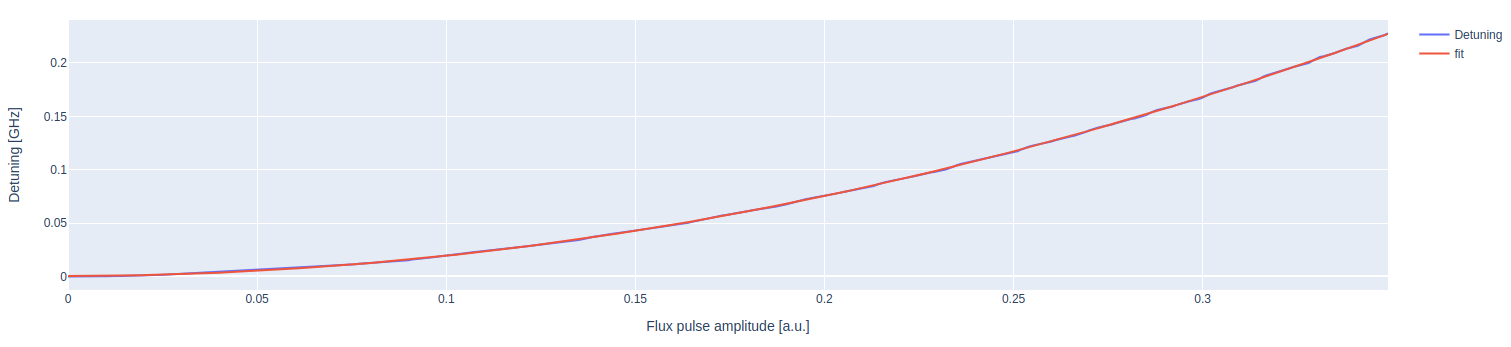
\includegraphics[width=\textwidth]{figures/png/flux_amp_freq.png}
    \caption{Expected output of the \tt{flux\_amplitude\_frequency} routine. Results obtained by executing the protocol on qubit \tt{B2}}
    \label{fig:flux_amplitude_frequency}
\end{figure}

It is important to note that the choice of \tt{amplitude\_step} must be sufficiently small to ensure accurate sampling of the $\langle X(t) \rangle$ and $\langle Y(t) \rangle$ traces. 
If the step size is too large, the oscillatory signals may be undersampled, leading to poor phase extraction and unreliable fit results, as illustrated in Figure \ref{fig:bad_sampling}.

\begin{figure}[h!]
    \centering
    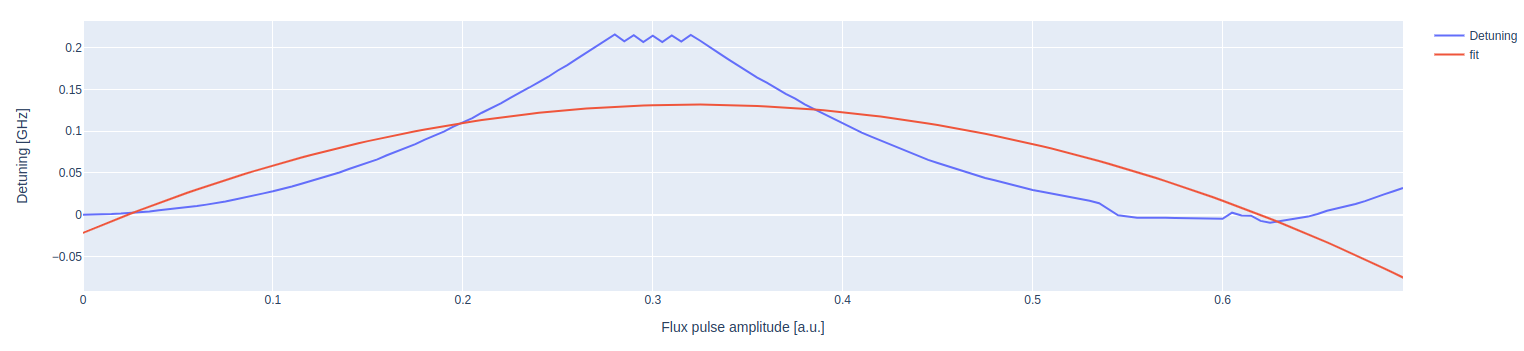
\includegraphics[width=\textwidth]{figures/png/low_sampling.png}
    \caption{Example of failed \tt{flux\_amplitude\_frequency} routine due to large amplitude step size. Results obtained by executing the protocol on qubit \tt{B4}}
    \label{fig:bad_sampling}
\end{figure}